\documentclass[aspectratio=169]{beamer}

\usetheme{Madrid}

\usepackage[T1]{fontenc}
\usepackage{amsmath,amssymb}
\usepackage{graphicx}
\usepackage{booktabs}
\usepackage{tikz}
%\usepackage{textcomp}
\usepackage{siunitx}

\usetikzlibrary{
	positioning,
	arrows.meta,
	shapes.geometric,
	fit,
	shadows
}

\title{WP3: Filtering and Clustering of AI-Generated Enzyme Mimics}
\author{}
\date{}

\begin{document}
	
	%------------------------------------------------
	\begin{frame}
		\titlepage
	\end{frame}
	
	%------------------------------------------------
	\begin{frame}{Motivation}
		
		\begin{itemize}
			\item Modern AI-based enzyme design pipelines can generate thousands of enzyme candidates.
			
			\vspace{0.2cm}
			
			\item Experimental validation is expensive and time-consuming.
			
			\vspace{0.2cm}
			
			\item Most generated structures exhibit limited structural diversity.
			
			\vspace{0.2cm}
			
			\item \textbf{Goal of WP3:}
			
			\begin{itemize}
				\item Preserve catalytic functionality;
				\item Maximize structural diversity;
				\item Select only the most promising candidates for laboratory validation.
			\end{itemize}
		\end{itemize}
		
	\end{frame}
	
	%------------------------------------------------
	\begin{frame}{Position of WP3 within the Workflow}
		
		\centering
		
		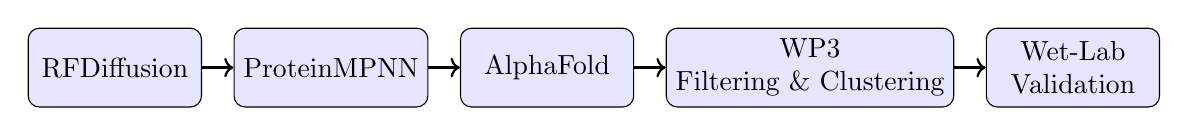
\begin{tikzpicture}[
			node distance=0.4cm,
			block/.style={
				draw,
				rounded corners,
				fill=blue!10,
				minimum width=2.2cm,
				minimum height=1cm,
				align=center
			},
			arrow/.style={->,thick}
			]
			
			\node[block] (rf) {RFDiffusion};
			
			\node[block,right=of rf] (mpnn)
			{ProteinMPNN};
			
			\node[block,right=of mpnn] (af)
			{AlphaFold};
			
			\node[block,right=of af] (fc)
			{WP3\\Filtering \& Clustering};
			
			\node[block,right=of fc] (lab)
			{Wet-Lab\\Validation};
			
			\draw[arrow] (rf)--(mpnn);
			\draw[arrow] (mpnn)--(af);
			\draw[arrow] (af)--(fc);
			\draw[arrow] (fc)--(lab);
			
		\end{tikzpicture}
		
		\vspace{0.8cm}
		
		\begin{center}
			Generate $\rightarrow$ Sequence Design $\rightarrow$ Structure Prediction
			$\rightarrow$ Candidate Selection $\rightarrow$ Experimental Validation
		\end{center}
		
	\end{frame}
	
	%------------------------------------------------
	\begin{frame}{WP3 Objectives}
		
		\begin{block}{Main Objective}
			Explore the structural space of enzyme mimics while preserving catalytic functionality.
		\end{block}
		
		\vspace{0.3cm}
		
		Two complementary strategies are employed:
		
		\begin{enumerate}
			\item \textbf{Filtering}
			\begin{itemize}
				\item Improve candidate quality.
				\item Remove unlikely functional structures.
			\end{itemize}
			
			\item \textbf{Clustering}
			\begin{itemize}
				\item Promote structural diversity.
				\item Ensure broad exploration of enzyme structural space.
			\end{itemize}
		\end{enumerate}
		
	\end{frame}
	
	%------------------------------------------------
	\begin{frame}{Protein Structure as a Graph}
		
		\begin{columns}
			
			\column{0.55\textwidth}
			
			\begin{itemize}
				\item Each amino-acid residue becomes a graph vertex.
				
				\item Residues are connected if their C$_\alpha$ atoms are spatially close.
				
				\item Threshold:
				\[
				\tau = 8 A\text{ (ångström unit)}
				\]
				
				\item Produces a residue interaction graph.
			\end{itemize}
			
			\[
			(v_i,v_j)\in E
			\iff
			\|\mathbf{x}_i-\mathbf{x}_j\|_2 \leq 8 \mathrm{A}
			\]
			
			\column{0.40\textwidth}
			
			\begin{center}
				\includegraphics[width=\linewidth]{enzyme\_mimicB1-501-379-00EN379a\_B1-501-379-00-enzyme\_mimicB1-501-379-00EN379a-ranked\_0.png}
			\end{center}
			
		\end{columns}
		
	\end{frame}
	
	%------------------------------------------------
	\begin{frame}{Graph-Based Structural Features}
		
		\small
		
		\begin{columns}
			
			\column{0.5\textwidth}
			
			\textbf{Basic Features}
			
			\begin{itemize}
				\item Number of nodes
				\item Number of edges
				\item Density
				\item Average degree
				\item Minimum degree
				\item Maximum degree
			\end{itemize}
			
			\vspace{0.3cm}
			
			\textbf{Connectivity Features}
			
			\begin{itemize}
				\item Connected components
				\item Diameter
				\item Average shortest path
			\end{itemize}
			
			\column{0.5\textwidth}
			
			\textbf{Topological Features}
			
			\begin{itemize}
				\item Clustering coefficient
				\item Degree centrality
			\end{itemize}
			
			\vspace{0.3cm}
			
			\textbf{Advanced Features}
			
			\begin{itemize}
				\item Catalytic residue geometry
				\item Minimum Dominating Set size
				\item Protein language model embeddings
				\item Structural descriptors
			\end{itemize}
			
		\end{columns}
		
	\end{frame}
	
	%------------------------------------------------
	\begin{frame}{Filtering Pipeline}
		
		\centering
		
		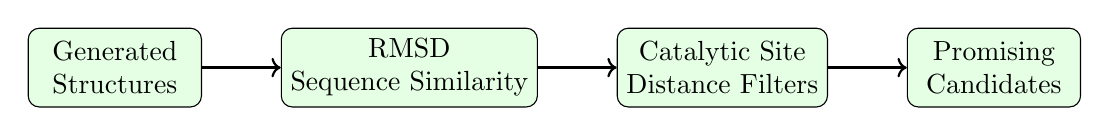
\begin{tikzpicture}[
			block/.style={
				draw,
				rounded corners,
				fill=green!10,
				minimum width=2.2cm,
				minimum height=1cm,
				align=center
			},
			arrow/.style={->,thick}
			]
			
			\node[block] (cand)
			{Generated\\Structures};
			
			\node[block,right=1cm of cand] (rmsd)
			{RMSD\\Sequence Similarity};
			
			\node[block,right=1cm of rmsd] (active)
			{Catalytic Site\\Distance Filters};
			
			\node[block,right=1cm of active] (survive)
			{Promising\\Candidates};
			
			\draw[arrow] (cand)--(rmsd);
			\draw[arrow] (rmsd)--(active);
			\draw[arrow] (active)--(survive);
			
		\end{tikzpicture}
		
		\vspace{0.8cm}
		
		\begin{itemize}
			\item Remove structurally implausible candidates.
			\item Preserve catalytic residue organization.
			\item Focus computational resources on promising structures.
		\end{itemize}
		
	\end{frame}
	
	%------------------------------------------------
	\begin{frame}{Active Site Preservation Filters}
		
		\textbf{Catalytic triad of turboPETase}
		
		\[
		SER - HIS - ASP
		\]
		
		\vspace{0.5cm}
		
		\textbf{Filter 1}
		
		\begin{itemize}
			\item Compare catalytic residue positions between generated and reference enzymes.
		\end{itemize}
		
		\vspace{0.3cm}
		
		\textbf{Filter 2}
		
		\begin{itemize}
			\item Measure internal distances:
			\begin{itemize}
				\item SER--HIS
				\item HIS--ASP
			\end{itemize}
		\end{itemize}
		
		\vspace{0.3cm}
		
		\textbf{Objective}
		
		\begin{itemize}
			\item Preserve catalytic geometry.
			\item Increase likelihood of catalytic functionality.
		\end{itemize}
		
	\end{frame}
	
	%------------------------------------------------
	\begin{frame}{Clustering Pipeline}
		
		\centering
		
		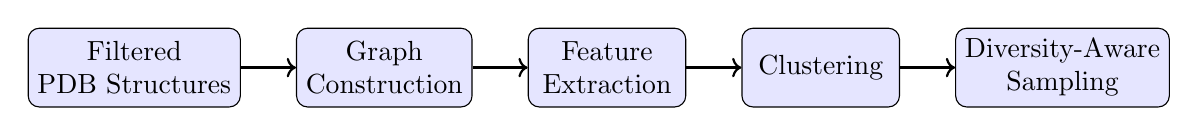
\begin{tikzpicture}[
			node distance=0.7cm,
			block/.style={
				draw,
				rounded corners,
				fill=blue!10,
				minimum width=2.0cm,
				minimum height=1cm,
				align=center
			},
			arrow/.style={->,thick}
			]
			
			\node[block] (pdb)
			{Filtered\\PDB Structures};
			
			\node[block,right=of pdb] (graph)
			{Graph\\Construction};
			
			\node[block,right=of graph] (feat)
			{Feature\\Extraction};
			
			\node[block,right=of feat] (cluster)
			{Clustering};
			
			\node[block,right=of cluster] (sample)
			{Diversity-Aware\\Sampling};
			
			\draw[arrow] (pdb)--(graph);
			\draw[arrow] (graph)--(feat);
			\draw[arrow] (feat)--(cluster);
			\draw[arrow] (cluster)--(sample);
			
		\end{tikzpicture}
		
		\vspace{1cm}
		
		\begin{enumerate}
			\item Convert structures into graphs.
			\item Compute structural descriptors.
			\item Build feature space.
			\item Identify structural families.
			\item Select representatives from each cluster.
		\end{enumerate}
		
	\end{frame}
	
	%------------------------------------------------
	\begin{frame}{Clustering Methods}
		
		\begin{itemize}
			\item K-Means
			\item Hierarchical Clustering
			\item Spectral Clustering
			\item Density-Based Clustering
		\end{itemize}
		
		\vspace{0.5cm}
		
		\textbf{Cluster quality metrics}
		
		\begin{itemize}
			\item Silhouette score
			\item Intra-cluster similarity
			\item Inter-cluster separation
		\end{itemize}
		
		\vspace{0.5cm}
		
		\textbf{Expected Outcome}
		
		\begin{itemize}
			\item Distinct structural families of enzyme mimics.
		\end{itemize}
		
	\end{frame}
	
	%------------------------------------------------
	\begin{frame}{Feature Space Representation}
		
		\centering
		
		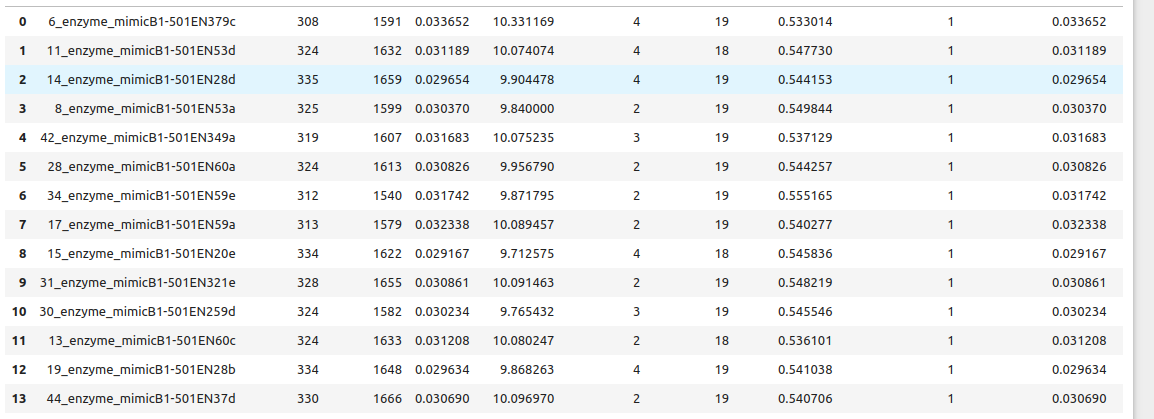
\includegraphics[width=0.9\textwidth]{structure_feature_space.png}
		
		\vspace{0.3cm}
		
		Protein structures represented through graph-based and biochemical descriptors.
		
	\end{frame}
	
	%------------------------------------------------
	\begin{frame}{K-Means Analysis}
		
		\begin{columns}
			
			\column{0.5\textwidth}
			
			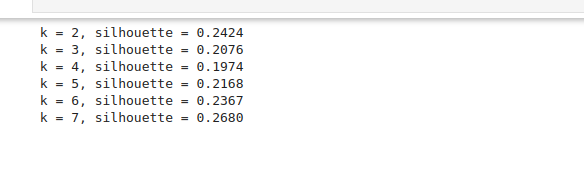
\includegraphics[width=\linewidth]{k_vals.png}
			
			\small
			
			Silhouette analysis used to determine the number of clusters.
			
			\column{0.5\textwidth}
			
			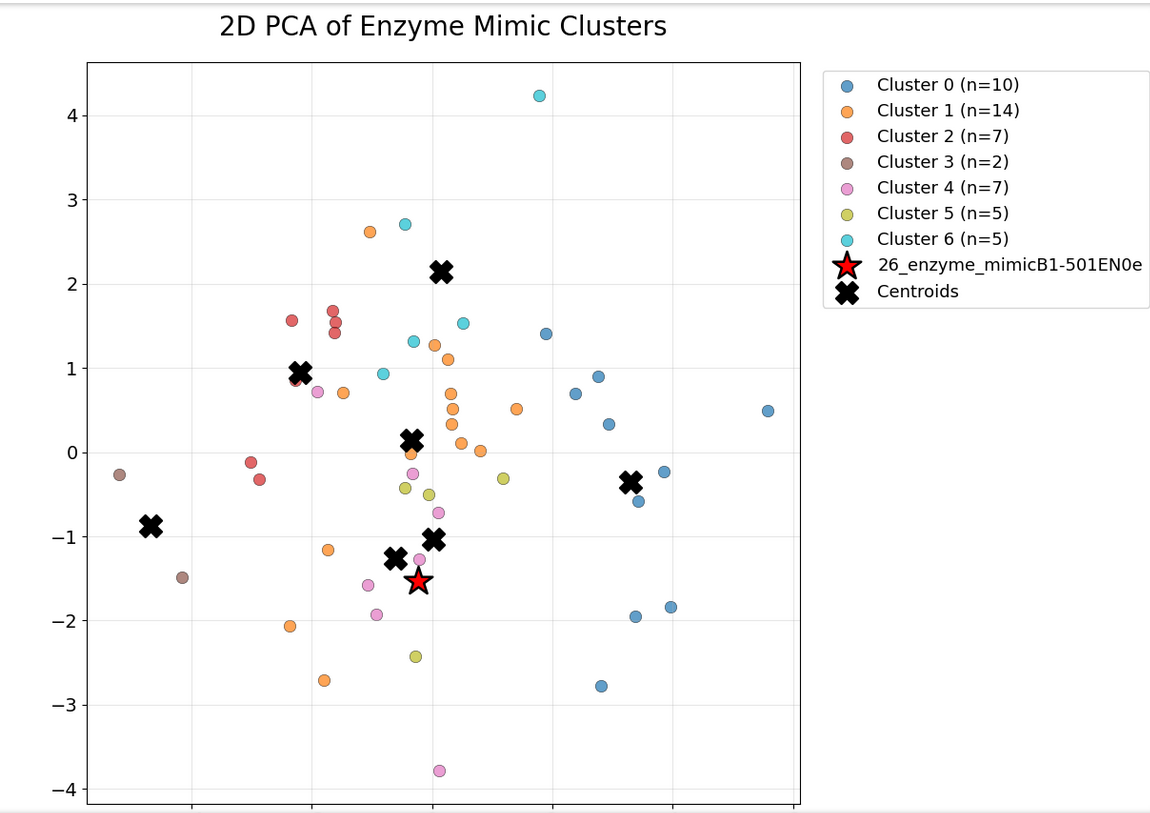
\includegraphics[width=\linewidth]{cluster_2dPCA.png}
			
			\small
			
			2D PCA visualization of clustered enzyme structures.
			
		\end{columns}
		
	\end{frame}
	
	%------------------------------------------------
	\begin{frame}{Consensus-Based Candidate Selection}
		
		\centering
		
		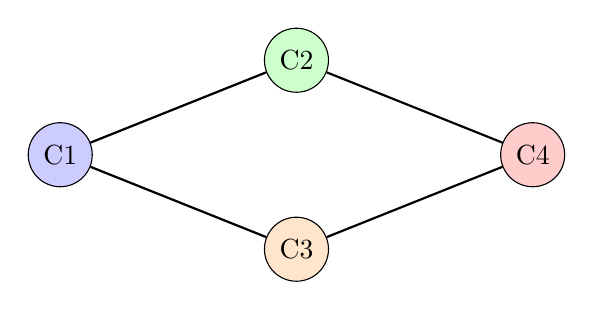
\begin{tikzpicture}
			
			\node[draw,circle,fill=blue!20] (c1) at (0,0) {C1};
			\node[draw,circle,fill=green!20] (c2) at (3,1.2) {C2};
			\node[draw,circle,fill=orange!20] (c3) at (3,-1.2) {C3};
			\node[draw,circle,fill=red!20] (c4) at (6,0) {C4};
			
			\draw[thick] (c1)--(c2);
			\draw[thick] (c1)--(c3);
			\draw[thick] (c2)--(c4);
			\draw[thick] (c3)--(c4);
			
		\end{tikzpicture}
		
		\vspace{0.7cm}
		
		\begin{itemize}
			\item Select representative structures from each cluster.
			\item Avoid selecting many variants of the same fold.
			\item Increase structural diversity of experimentally tested candidates.
		\end{itemize}
		
	\end{frame}
	
	%------------------------------------------------
	\begin{frame}{Expected Impact}
		
		\begin{itemize}
			\item Reduce wet-lab validation costs.
			
			\item Increase structural diversity of enzyme mimics.
			
			\item Preserve catalytic functionality.
			
			\item Introduce graph-theoretical and combinatorial descriptors into enzyme design.
			
			\item Enable systematic exploration of protein structural space.
			
			\item Establish a feedback loop between AI generation and experimental validation.
		\end{itemize}
		
		\vspace{0.8cm}
		
		\begin{center}
			\Large
			Towards Reliable and Diverse AI-Generated Enzymes
		\end{center}
		
	\end{frame}
	
	%------------------------------------------------
\end{document}